
In addition to \acp{SEP}, extremely high-energy \acp{GCR} dominated by protons and albedo particles generated through the interaction between \acp{GCR} and the lunar regolith are two other crucial components of the plasma environment that cause radiation hazard on the lunar surfaces.
Unlike Earth, with a thick atmosphere and a global magnetosphere acting as energy cutoffs for energetic particles and filters of the radiation hazard, the Moon lacks those protections. As a result, it is well known that the \ac{GCR} flux of energy above a few MeV on the lunar surface is identical to that in deep space.

However, during the recent solar minimum period over July 2019 - July 2020, solar eruptions were rare on the solar surface, and so were \acp{SEP}. According to the measurement from \ac{LND}, no \ac{SEP} events with energy exceeding ten MeV arrives at the lunar surface during its operation time.
Therefore, it is an excellent opportunity to study the variation of \acs{GCR} without the interference of \acp{SEP}, especially during this unusual solar minimum \citep{Strauss2023ApJ, Fu2021ApJS} and validate the new instrument's performance and response to those high energetic particles.    

Furthermore, albedo protons, which emitted from the lunar regolith and move upward, represent a significant contribution to the radiation hazard on the lunar surface and can potentially be used to detect the hydrogen material in the lunar regolith since the flux of albedo proton depends on the regolith composition and the \ac{GCR} flux \citep{Schwadron2016Icarus}.
Below 50 MeV, the flux of albedo proton surpasses that of \ac{GCR} protons on the lunar surface \citep{Dobynde2021JGRE, Wimmer2020SSRv}, and their energy can reach hundreds of MeV, posing a risk to biological tissue and electronic devices.

Benefiting from the advanced structure of \ac{LND}'s charged particle telescope, we have designed data products based on the Xmas plot (See instrument chapter and the following content for details) and successfully obtained the first measurement of albedo proton flux in the energy range between 65 and 75 MeV on the lunar surface.

\\


\subsection*{Short overview of the publication}\\

We first give a detailed explanation of the instrument's inner structure and measurement principle. Especially configuration changes during the first year of the mission are explained. The simulation set-up and the Xmas plot which summarizes primary data products are the basis of the study and are explained.
With the help of the \ac{Geant4} simulation and the \ac{GCR} model, we carefully calibrate the data product and remove the background noise due to the contamination of other particles. As a result, we obtain a spectrum of \ac{GCR} proton and flux of albedo protons on the lunar surface. Finally, we compare the measurement with the prediction from the \ac{REDMoon} model and the measurement from other instruments and discuss the possible implication of the measurement.
This work attempts to answer questions, C1, C2, C3, and C5,regarding the cosmic rays and its induced secondary particles .

\begin{itemize}
    \item   In this paper, the new primary protons products, based on the penetrating protons, are for the first time presented. They extend the proton data coverage to a few hundred MeV and measure the lower energy \ac{GCR} protons. The flux of the albedo proton with an energy of approximately 70 MeV is measured for the first time on the lunar surface. Possible instrumental contamination and background noise are properly removed.
    \item The \ac{LND} \ac{GCR} spectrum is consistent with \ac{SOHO}/\ac{EPHIN} measurement between 10 - 50 MeV.  Predictions from CREME96 \citep{Tylka1997ITNS} \ac{GCR} model are approximately 50 \% lower than measurements during solar activity minimum periods.
    \item  The albedo proton flux agrees with the \ac{LRO}/\ac{CRaTER} measurement between 50 - 150 MeV and is consistent with the model prediction by the \ac{REDMoon} model.
    \item We derived the ratio of albedo to primary protons flux at the same energy from observation and simulation. We found that the ratio peaks at 20 MeV with a value exceeding 2. The ratio decreases quickly with the increase of energy.
\end{itemize}




The following article is reproduced from \textcite{Xu-2022-LND-GCRalbedo}, which is an open-access article reproducted under the terms of 
the CC-BY license. The supplement material including the configuration changes of LND up to now and the data we used in the main content is attached afterward. 
\\

\noindent\pubcite{Xu-2022-LND-GCRalbedo}\\
\strut\hfill Own contribution: 90\%

\newpage
\newcounter{includepdfpageFrontierTwentyTwo}

\addtocounter{subsection}{1}
\setcounter{subsubsection}{1} 
\phantomsection
\addcontentsline{toc}{subsection}{\arabic{chapter}.\arabic{section}.\arabic{subsection} Primary and albedo protons detected by the Lunar Lander Neutron and Dosimetry experiment on the lunar farside(Publication Frontier in Astronomy and Space Sciences 2022)}
%
\phantomsection
\addcontentsline{toc}{subsubsection}{\arabic{chapter}.\arabic{section}.\arabic{subsection}.\arabic{subsubsection} Introduction}
\label{sec:paper_xu2022}
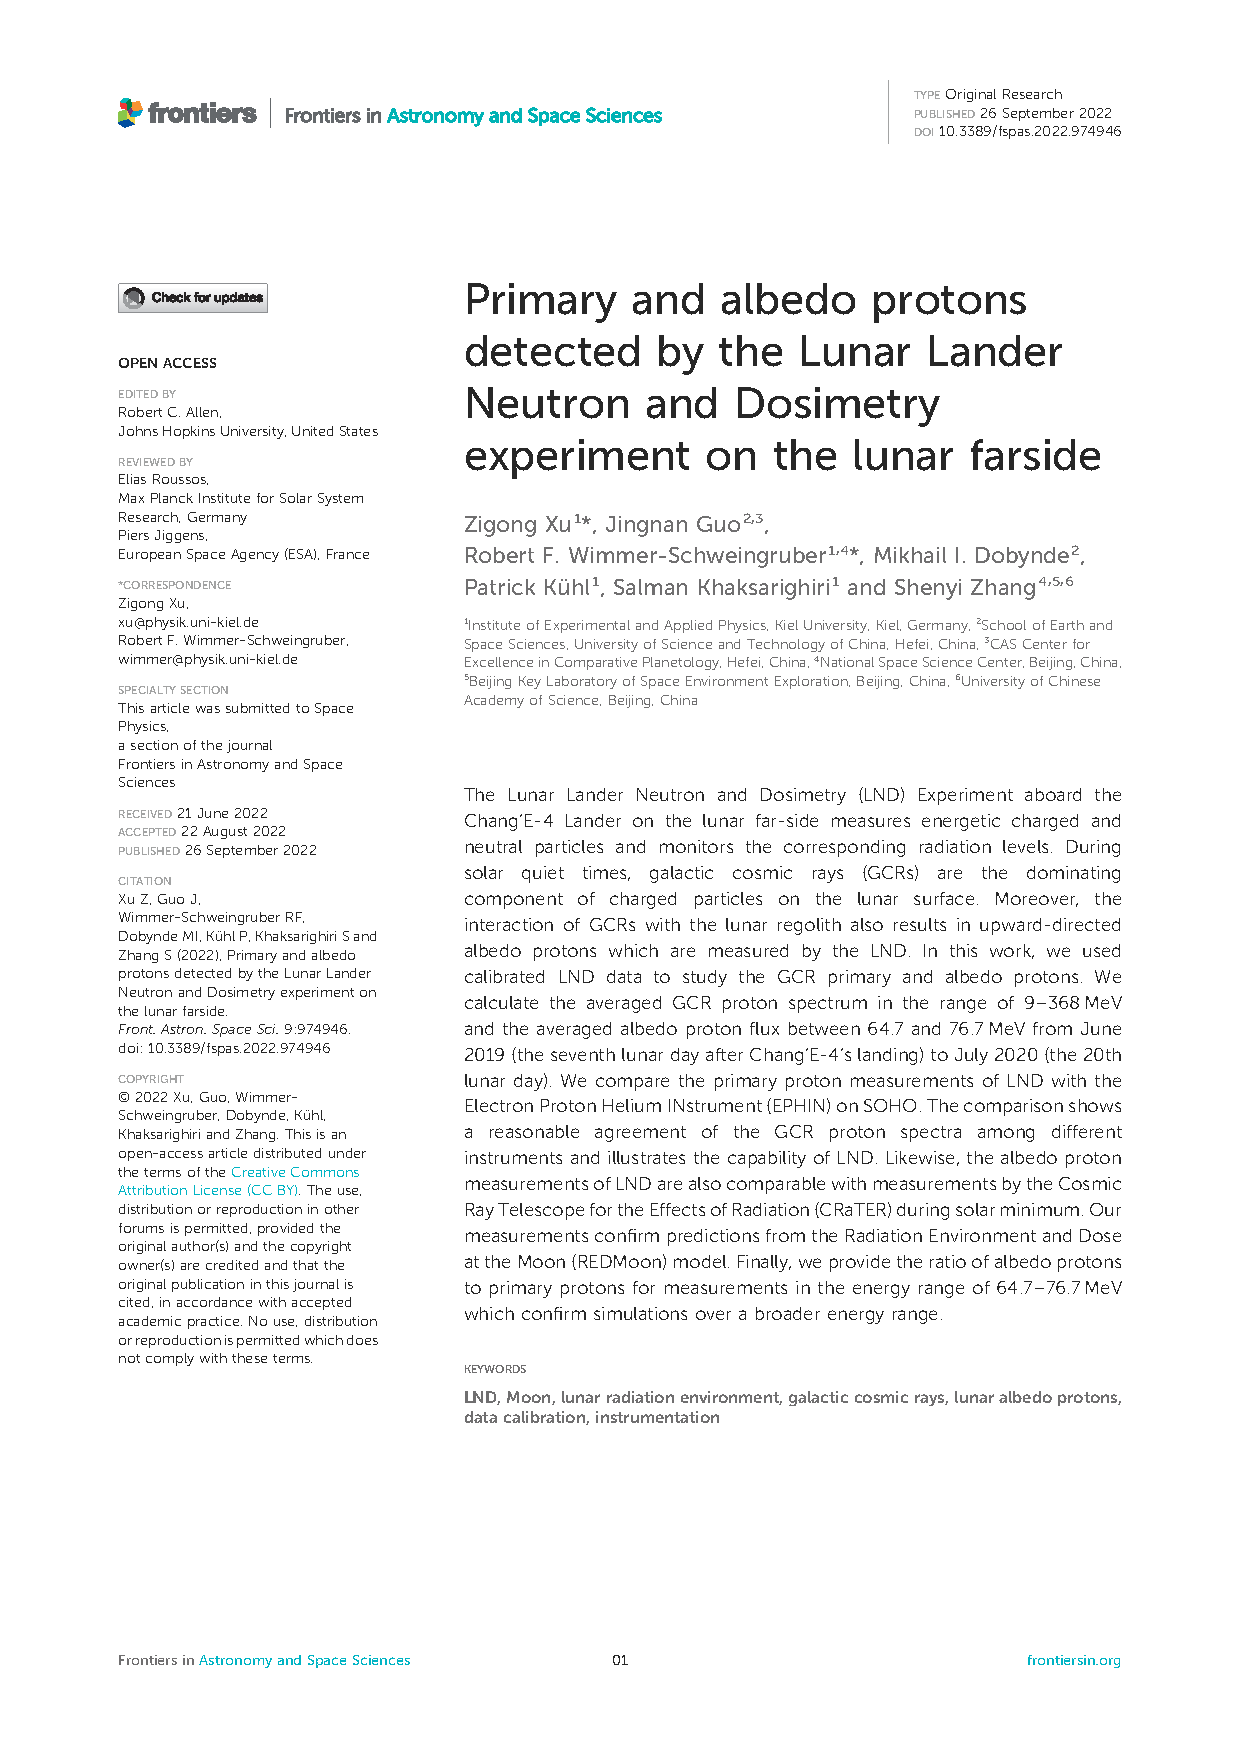
\includepdf[pages={1-3}, link, linkname=paper_xu2022, scale=.9, pagecommand={\refstepcounter{includepdfpageFrontierTwentyTwo}\label{paper_xu2022.\theincludepdfpageFrontierTwentyTwo}}]{publications/Xu_et_al_2022_Frontier.pdf}
%
\addtocounter{subsubsection}{1} 
\phantomsection
\addcontentsline{toc}{subsubsection}{\arabic{chapter}.\arabic{section}.\arabic{subsection}.\arabic{subsubsection} Preparation of LND data}
\includepdf[pages={4-8}, link, linkname=paper_xu2022, scale=.9, pagecommand={\refstepcounter{includepdfpageFrontierTwentyTwo}\label{paper_xu2022.\theincludepdfpageFrontierTwentyTwo}}]{publications/Xu_et_al_2022_Frontier.pdf}
%
\addtocounter{subsubsection}{1} 
\phantomsection
\addcontentsline{toc}{subsubsection}{\arabic{chapter}.\arabic{section}.\arabic{subsection}.\arabic{subsubsection} Measurements and comparison with model}
\includepdf[pages={9-11}, link, linkname=paper_xu2022, scale=.9, pagecommand={\refstepcounter{includepdfpageFrontierTwentyTwo}\label{paper_xu2022.\theincludepdfpageFrontierTwentyTwo}}]{publications/Xu_et_al_2022_Frontier.pdf}
%
\addtocounter{subsubsection}{1} 
\phantomsection
\addcontentsline{toc}{subsubsection}{\arabic{chapter}.\arabic{section}.\arabic{subsection}.\arabic{subsubsection} Summary, discussion and conclusion}
\includepdf[pages={12}, link, linkname=paper_xu2022, scale=.9, pagecommand={\refstepcounter{includepdfpageFrontierTwentyTwo}\label{paper_xu2022.\theincludepdfpageFrontierTwentyTwo}}]{publications/Xu_et_al_2022_Frontier.pdf}
%
\addtocounter{subsubsection}{1} 
\phantomsection
\addcontentsline{toc}{subsubsection}{\arabic{chapter}.\arabic{section}.\arabic{subsection}.\arabic{subsubsection} References}
\includepdf[pages={13-14}, link, linkname=paper_xu2022, scale=.9, pagecommand={\refstepcounter{includepdfpageFrontierTwentyTwo}\label{paper_xu2022.\theincludepdfpageFrontierTwentyTwo}}]{publications/Xu_et_al_2022_Frontier.pdf}
%
\addtocounter{subsubsection}{1} 
\phantomsection
\addcontentsline{toc}{subsubsection}{\arabic{chapter}.\arabic{section}.\arabic{subsection}.\arabic{subsubsection} Supplement material}
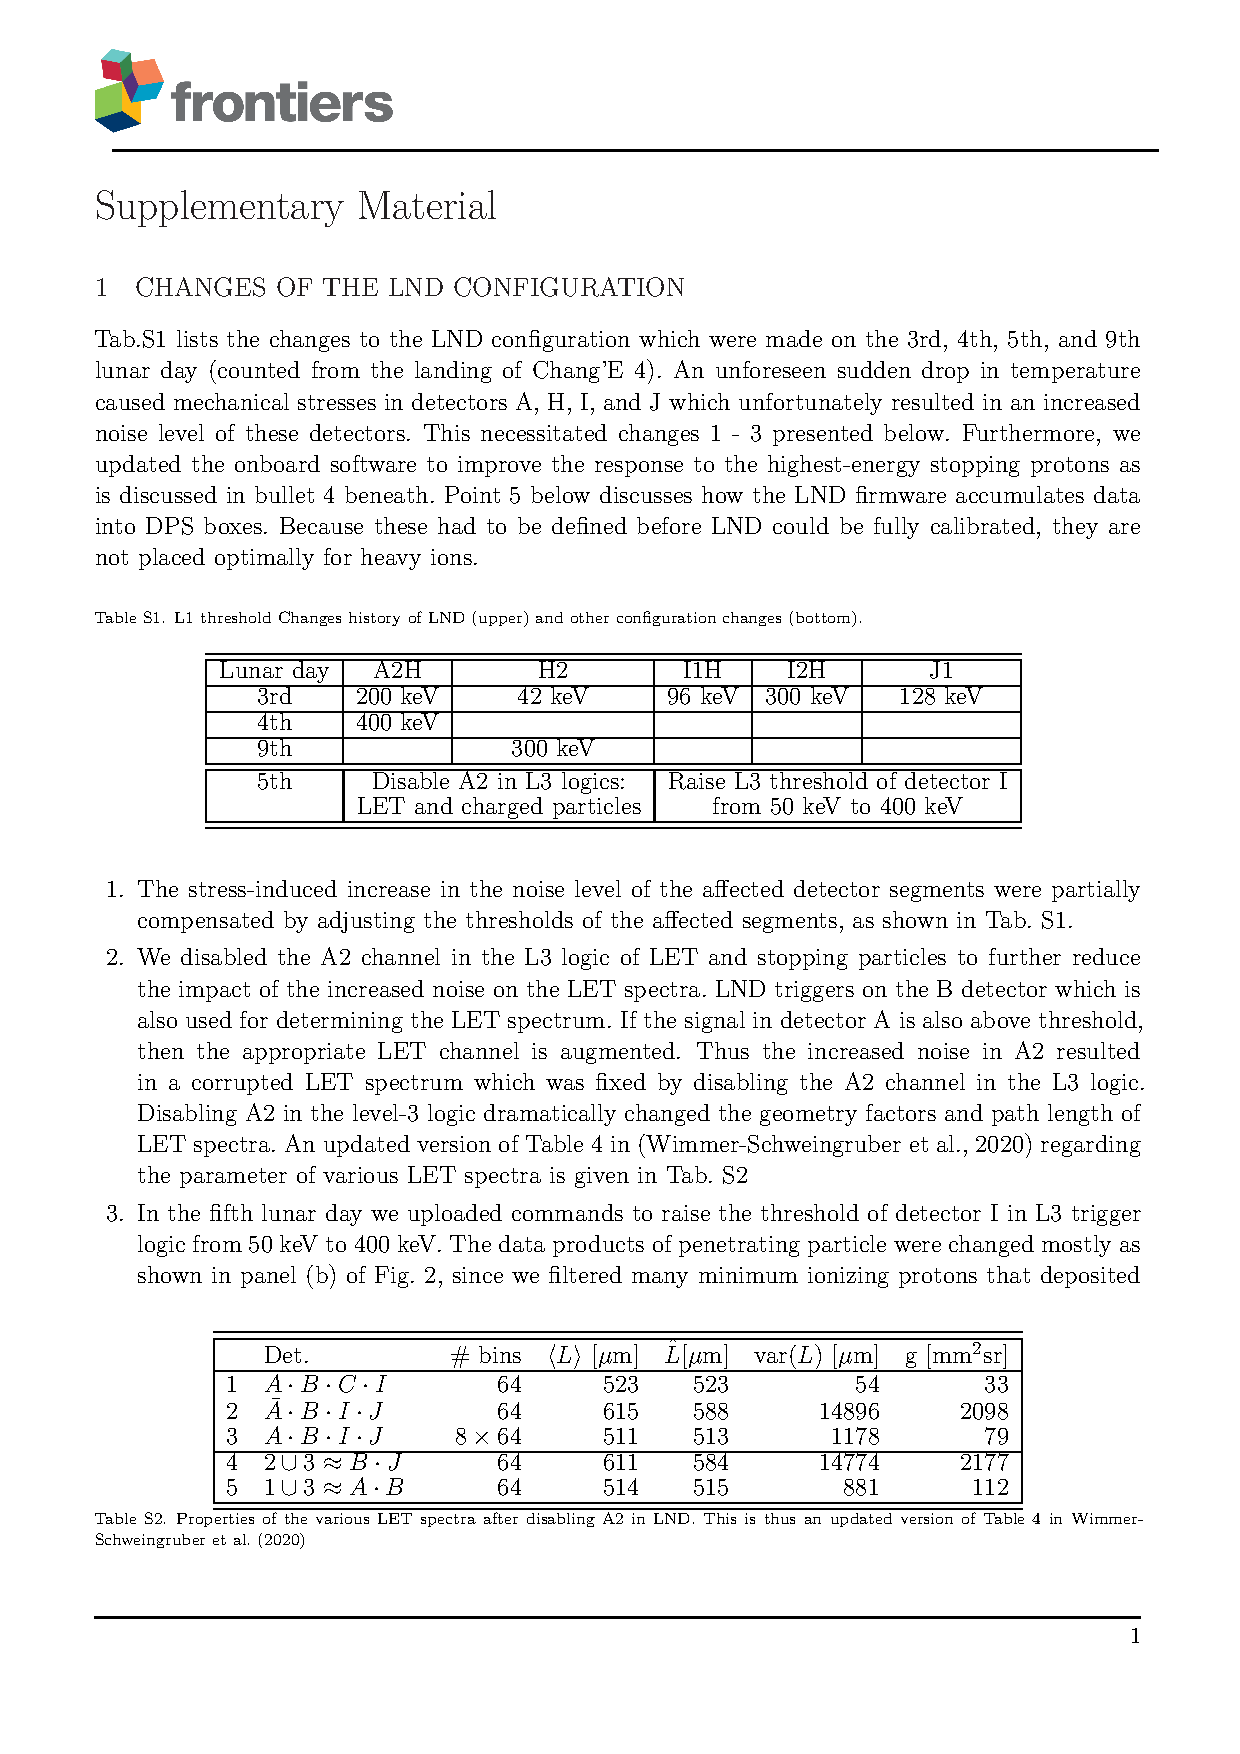
\includepdf[pages={1-3}, link, linkname=paper_xu2022, scale=.9, pagecommand={\refstepcounter{includepdfpageFrontierTwentyTwo}\label{paper_xu2022.\theincludepdfpageFrontierTwentyTwo}}]{publications/Xu_et_al_2022_frontier_appendix.pdf}